\chapter{Testes e Resultados}\label{cap:testes_e_resultados}
Neste capítulo são descritos os testes de desenvolvimento e performance do aplicativo. Além disso, contém também uma descrição dos resultados dos testes práticos com crianças.

\section{Testes de Desenvolvimento}

Nesta seção são detalhados os testes de desenvolvimento e performance do software de reconhecimento dos blocos.


\subsection{\textbf{Teste de Tempo de Resposta do Reconhecimento}}

Após o término do desenvolvimento do protótipo, foram realizados testes para mensurar o tempo médio de resposta do algoritmo de reconhecimento por quantidade de blocos. A metodologia adotada para esse teste foi capturar uma amostra de imagens contendo 1 bloco, 2 blocos e 3 blocos, separados em blocos normais e númericos como ilustrado na Figura \ref{figura:ttr}. Por meio dessas imagens, foram realizadas 50 medições do tempo de resposta do algoritmo de reconhecimento por quantidade de blocos, isto é, 50 medições das imagens com apenas 1 bloco, 50 medições das imagens com 2 blocos e por fim 50 medições das imagens com 3 blocos. Após todos os valores coletados, foi calculada uma média simples por quantidade de blocos e por tipo de bloco a fim de diminuir possíveis eventualidades que pudessem provocar alterações no tempo de resposta. O objetivo deste teste é verificar se há diferença no tempo de resposta entre blocos normais e blocos numéricos, sendo que estes passam pela etapa de reconhecimento óptico de caracteres.

\begin{figure}[H]
    \caption{Exemplos de imagens para teste de tempo de resposta}
    \centering
    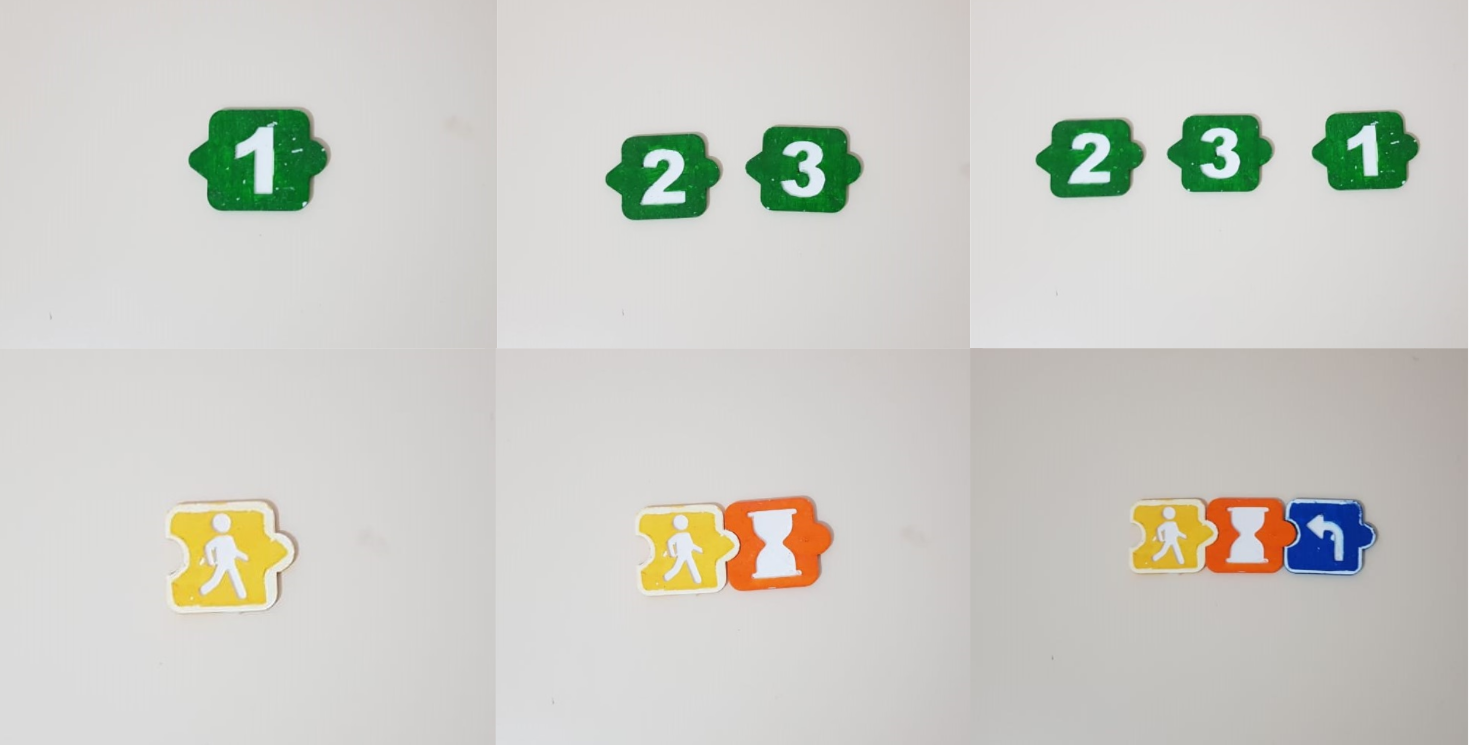
\includegraphics[width=15cm]{Imagens/Cap5/ttr.png}
    \legend{\small{Fonte: os autores (2020)}}
    \label{figura:ttr}
\end{figure}

Como pode-se ver na tabela \ref{table:tempo_resposta} e no gráfico ilustrado na Figura \ref{figura:ttr_grafico} que derivam do resultado do teste de tempos de resposta, existe uma diferença considerável no tempo de resposta entre blocos normais e blocos numéricos e essa diferença tende a crescer considerando o acréscimo de blocos numéricos. Pode-se notar também que o tempo de resposta dos blocos normais tende a se manter estável mesmo com a inserção de mais blocos normais. Porém, pode-se notar também que o tempo de resposta tende a aumentar consideravelmente com o acréscimo de blocos numéricos. 

    \begin{table}[H]
        \centering
        \caption{Tempo(s) de resposta por quantidade e tipo de bloco }
        \label{table:tempo_resposta}
        \begin{tabular}{ |c|c|c| } 
         \hline
        Quantidade de Blocos & Blocos Normais & Blocos Numéricos \\
         \hline
        1 & 37.1ms & 427.7ms \\
         \hline
        2 & 39.8ms & 674.1ms\\
         \hline
        3 & 39.7ms & 987.1ms\\    [0.5ex]    
         \hline
        
        \end{tabular}
        \legend{\small{Fonte: os autores (2020)}}
    \end{table}

\begin{figure}[H]
    \caption{Gráfico tempo de resposta}
    \centering
    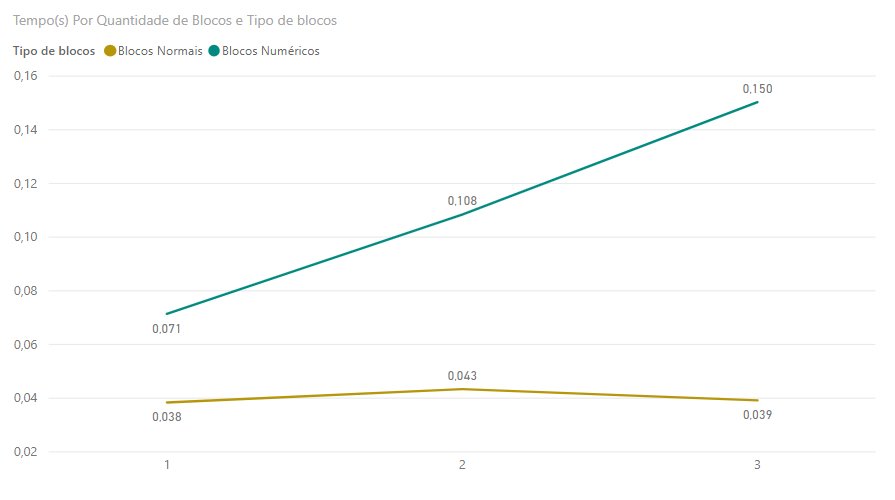
\includegraphics[width=14cm]{Imagens/Cap5/ttr_grafico.PNG}
    \legend{\small{Fonte: os autores (2020)}}
    \label{figura:ttr_grafico}
\end{figure}

\subsection{\textbf{Teste de Taxa de Acerto do Reconhecimento}}

Após o término do desenvolvimento do protótipo, foram realizados testes para mensurar a taxa de acerto do aplicativo em relação ao reconhecimento dos blocos. A metodologia adotada para esse teste foi capturar uma amostra de imagens de uma mesma sequência de blocos, das quais uma metade dessas imagens são capturadas com iluminação adequada e seguindo as recomendações do aplicativo jogo, e a outra metade das imagens capturadas com iluminação inadequada e sem seguir as recomendações de captura do aplicativo jogo. E, por meio dessas imagens, calcular as taxas de acerto para os dois tipos de imagens com o objetivo de verificar e mensurar a importância de usar o aplicativo jogo em um ambiente iluminado adequadamente e seguindo as recomendações do aplicativo jogo em relação à captura das imagens. Uma imagem considerada iluminada adequadamente é uma imagem que está sob  iluminação semelhante a iluminação utilizada para fazer a calibração do algoritmo de reconhecimento, e recomenda-se que a calibração seja realizada em um ambiente iluminado uniformemente com luz branca. 

Para o teste de taxa de acerto, foi coletado uma amostra de 200 imagens com blocos andar, esperar, virar e loop. Das 200 imagens, 100 imagens foram coletadas sob iluminação semelhante à utilizada na calibração do algoritmo e seguindo a orientação de tamanho sugerida na tela de captura de imagem do aplicativo jogo, como ilustrado na Figura \ref{figura:tta_boa}. As outras 100 imagens, foram coletadas sob iluminação diferente da utilizada para calibração, com distâncias diferentes das recomendadas pelo aplicativo jogo e sob trepidações no momento da captura, ou seja, imagens borradas, como ilustrado na Figura \ref{figura:tta_ruim}.

\begin{figure}[H]
    \caption{Imagens adequadas para teste taxa de acerto}
    \centering
    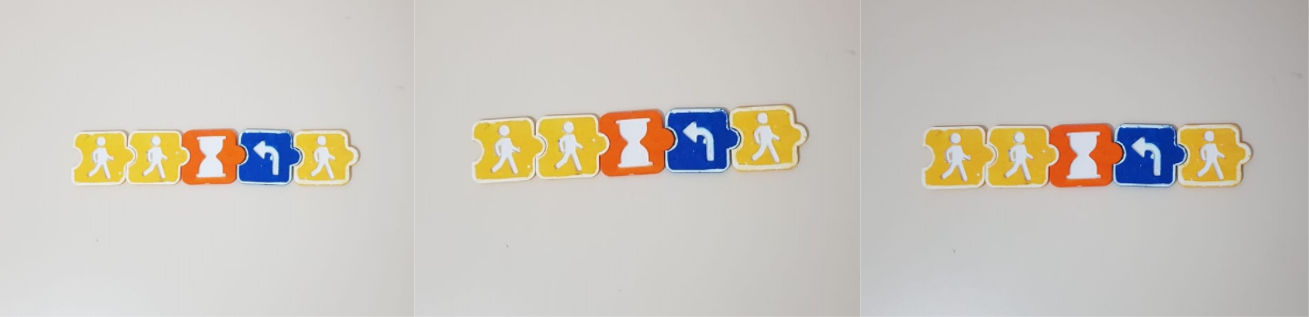
\includegraphics[width=15cm]{Imagens/Cap5/tta_boa.PNG}
    \legend{\small{Fonte: os autores (2020)}}
    \label{figura:tta_boa}
\end{figure}

\begin{figure}[H]
    \caption{Imagens não adequadas para teste de taxa de acerto}
    \centering
    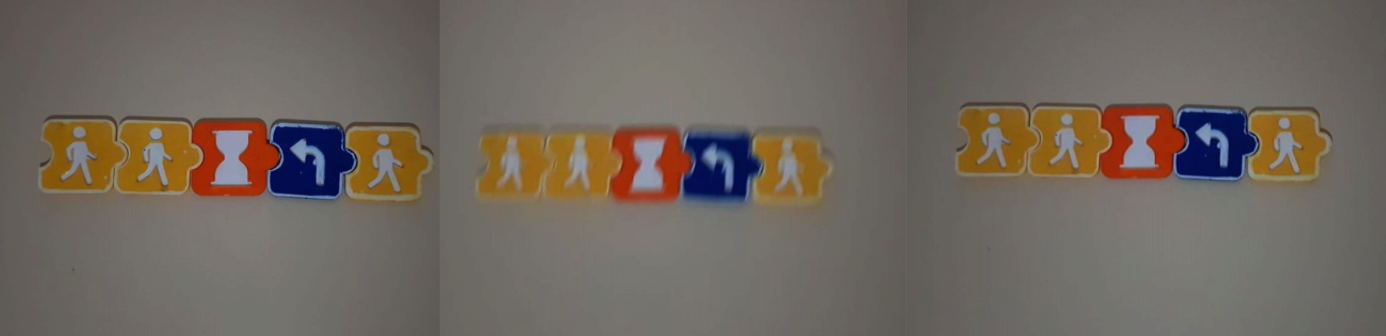
\includegraphics[width=15cm]{Imagens/Cap5/tta_ruim.PNG}
    \legend{\small{Fonte: os autores (2020)}}
    \label{figura:tta_ruim}
\end{figure}

O resultado do teste foi, das 100 imagens iluminadas adequadamente e capturadas sob as recomendações do aplicativo jogo, o algoritmo de reconhecimento acertou 92 das sequências dessas imagens, portanto obteve uma taxa de acerto de 92\%. Porém, das 100 imagens iluminadas inadequadamente e que não foram capturadas seguindo as recomendações do aplicativo, o algoritmo acertou apenas 58 sequências das 100 imagens, ou seja, obteve uma taxa de acerto de 58\%. Portanto, pode-se concluir que é fundamental que o aplicativo jogo seja utilizado em um ambiente adequadamente iluminado e seguindo as recomendações de captura de imagem a fim de garantir um bom funcionamento do aplicativo jogo.


\section{Testes Práticos}

Nesta seção são descritos os testes práticos com crianças.

\subsection{\textbf{Descrição}}


A metodologia de teste com crianças proposta pelos autores foi submetida e obteve a aprovação do comitê de ética, conforme parecer contido no Anexo A. Portanto, antes de iniciar as etapas descritas abaixo, foram apresentados aos participantes os objetivos e a metodologia da pesquisa. A participação foi  realizada apenas após a assinatura do Termo de Consentimento Livre e Esclarecido (TCLE) pelos responsáveis e pelo termo de assentimento assinado pela criança, ambos termos encontram-se no Apêndice A e no Apêndice B respectivamente. Os participante também receberam uma via do TCLE assinado pelo pesquisador responsável. Os dados pessoais coletados, como nome e idade, serão acessados apenas pela equipe de pesquisa. Todos os dados serão destruídos, no prazo de, no máximo, 1 ano.

Pensando nas eventualidades causadas pelo vírus Sars-CoV-2, causador da pandemia mundial do covid-19 no ano de 2020, os testes descritos abaixo foram realizados integralmente seguindo as orientações da OMS \cite{oms_2020} de prevenção ao Sars-CoV-2.

Os testes práticos foram realizados em duas etapas. A primeira etapa foi a resolução dos desafios propostos pelo jogo e a segunda etapa foi a resposta ao questionário de pesquisa criado pelos pesquisadores. A primeira etapa foi realizada pela criança e a segunda etapa pode ser realizada pela criança com, ou sem, o auxílio de um responsável que tenha acompanhado a aplicação da primeira etapa. Os testes foram realizados com 2 participantes.

Na primeira etapa os participantes jogaram o jogo dentro do ambiente de sua escolha. Os pesquisadores foram até o local de aplicação para disponibilizar os blocos físicos, celular com o aplicativo e explicar o funcionamento do jogo para os responsáveis e as crianças. A aplicação da primeira foi supervisionada pelos responsáveis e pesquisadores. Os participantes jogaram o  aplicativo jogo por um tempo entre 15 a 30 minutos.

Na segunda etapa do teste, o participante respondeu  a um questionário online que foi disponibilizado após o término da primeira etapa e ficou disponível por uma semana. O objetivo foi  validar a efetividade do aplicativo jogo em relação ao engajamento do participante, competência em ensinar programação e
capacidade de ensinar sobre reciclagem. Foi disponibilizado ao participante ou responsável, por meio do Whatsapp ou e-mail, o link do questionário. O questionário possui 5 perguntas obrigatórias e estima-se que o tempo de preenchimento do questionário seja de aproximadamente 15 minutos. As 2 primeiras perguntas são abertas, a pergunta 3 é binária com opções sim e não  e, nas perguntas 4 e 5, são mostradas ao respondente a imagem de um labirinto Figura \ref{figura:q4}, semelhante ao do jogo, e uma imagem de uma garrafa plástica Figura \ref{figura:q5} respectivamente, todas com 4 alternativas , das quais apenas uma é correta. 

\begin{enumerate}
    \item  Qual seu primeiro nome ? 
    
    \item Qual a sua idade ?
    
    \item Você se sentiu motivado a continuar jogando o jogo ?
    
    \item   Qual sequência corresponde a resolução do labirinto abaixo (Figura \ref{figura:q4}) ?
    
    \begin{figure}[H]
    \caption{Pergunta 4}
    \centering
    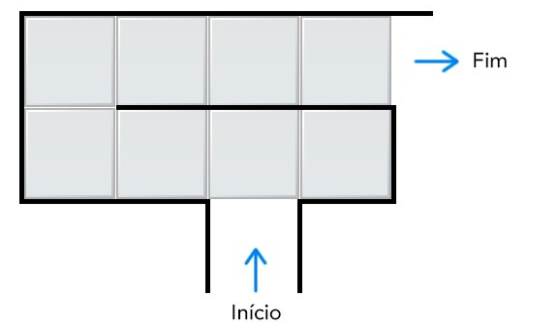
\includegraphics[width=10cm]{Imagens/Cap5/Q4.png}
    \legend{\small{Fonte: os autores (2020)}}
    \label{figura:q4}
    \end{figure}

     \begin{enumerate}
     \item $\uparrow,  \leftarrow, \uparrow, \rightarrow$;
     \item $\uparrow, \leftarrow, \leftarrow, \uparrow, \rightarrow, \rightarrow, \rightarrow, \rightarrow$;
     \item  $\uparrow, \leftarrow, \leftarrow, \uparrow, \rightarrow, \rightarrow, \rightarrow$;
     \item .$\leftarrow, \leftarrow, \uparrow, \rightarrow, \rightarrow, \rightarrow, \rightarrow$.
     \end{enumerate}

    \item   Em qual das lixeiras você descartaria o lixo abaixo (Figura \ref{figura:q5})?
    
    \begin{figure}[H]
        \caption{Pergunta 5}
        \centering
        
\includegraphics[width=8cm]{Imagens/Cap5/Q5.png}
        \legend{\small{Fonte: os autores (2020)}}
        \label{figura:q5}
    \end{figure}

     \begin{enumerate}
     \item Imagem de uma lixeira azul; 
     \item Imagem de uma lixeira amarela; 
     \item Imagem de uma lixeira vermelha; 
     \item Imagem de uma lixeira verde;
     \end{enumerate}


\end{enumerate}


\subsection{\textbf{Teste com Crianças}}
Os testes foram feitos com duas crianças, com 6 e 11 anos, em suas respectivas casas. Ambas as crianças apresentaram alto interesse no jogo e reportaram que gostariam de mais fases.  A Figura \ref{figura:teste_crianca_2} apresenta a criança 2 testando o jogo.

\begin{figure}[H]
    \caption{Teste com a Criança 2}
    \centering
    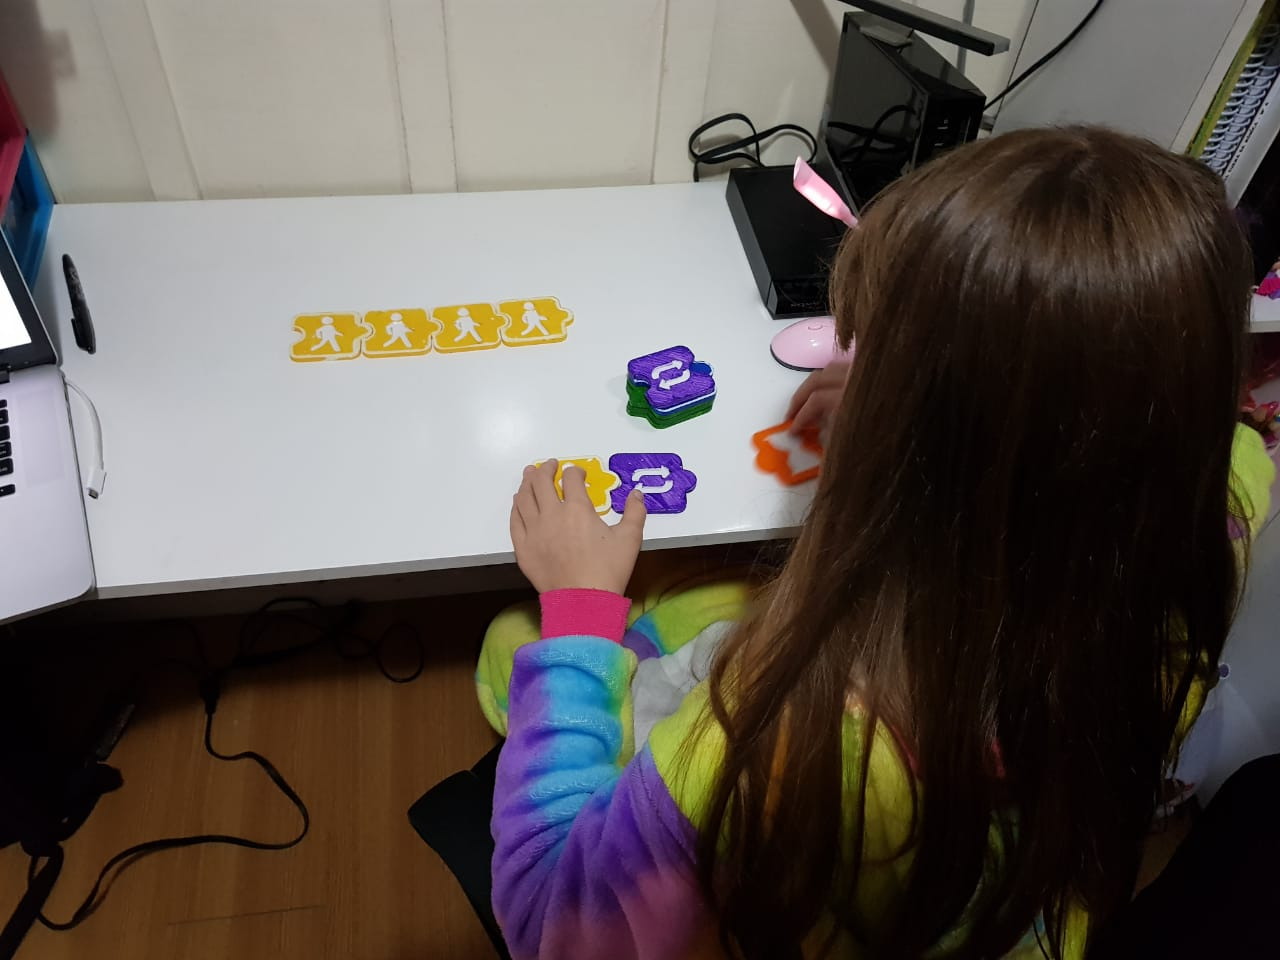
\includegraphics[width=\linewidth]{Imagens/Cap5/Teste_crianca_2.jpeg}
    \legend{\small{Fonte: os autores (2020)}}
    \label{figura:teste_crianca_2}
\end{figure}

Foi apresentado para as crianças o jogo e os blocos para que elas pudessem resolver os desafios e posteriormente foi aplicado o questionário para avaliação do jogo e do conhecimento obtido.

A Figura \ref{figura:solucao_crianca_1} apresenta a solução proposta pela criança 1 de um dos desafios apresentados.

\begin{figure}[H]
    \caption{Solução Criança 1}
    \centering
    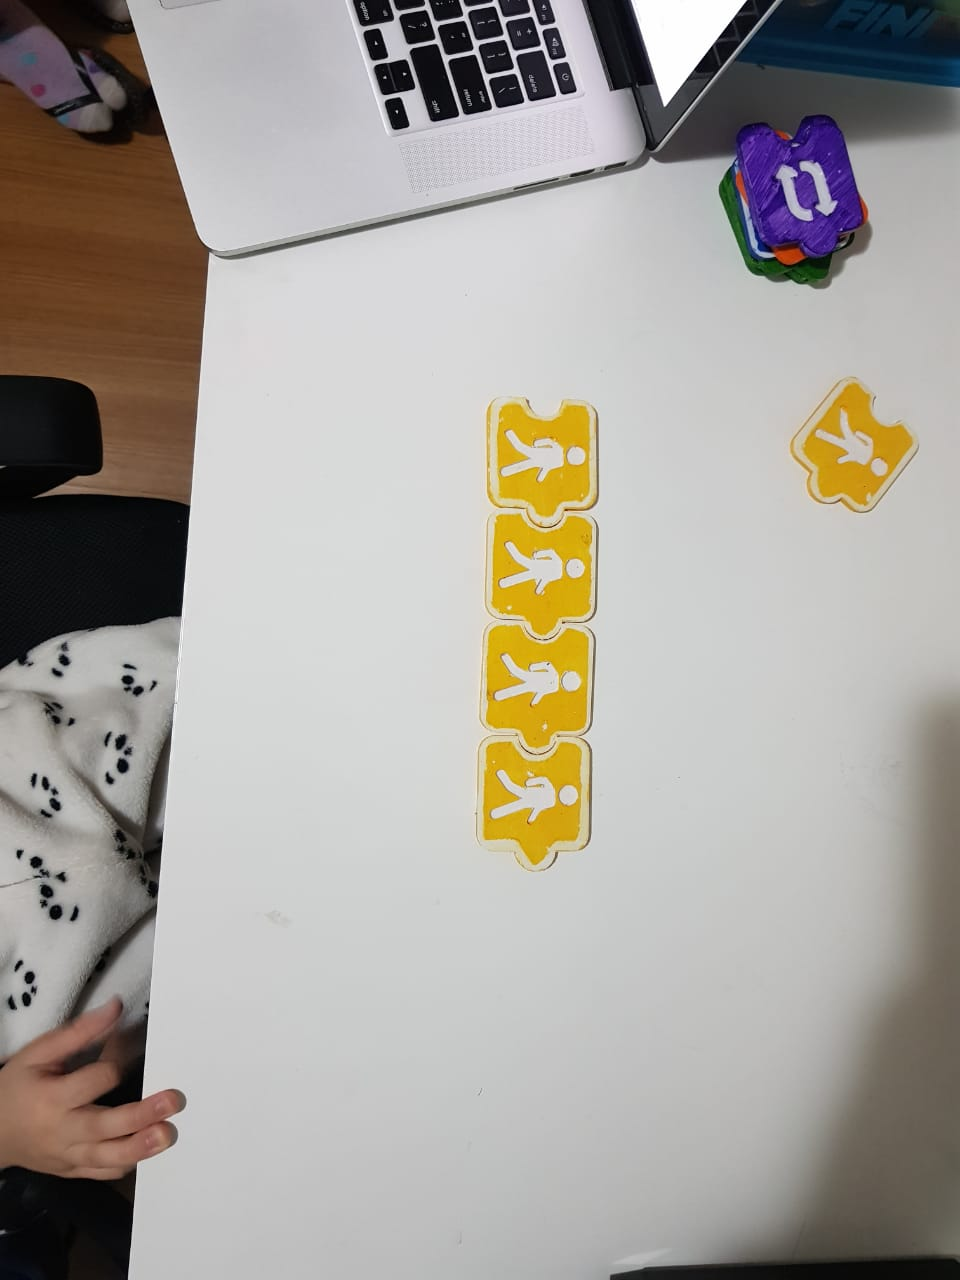
\includegraphics[width=\linewidth]{Imagens/Cap5/Teste_crianca_1.jpeg}
    \legend{\small{Fonte: os autores (2020)}}
    \label{figura:solucao_crianca_1}
\end{figure}

As subseções a seguir detalham como foi o procedimento de teste com cada uma das crianças.

\subsubsection{Criança 1}

Os testes foram realizados com uma criança de 6 anos, em sua casa no dia 04/11/2020. Primeiramente foi apresentado para a criança os blocos e o jogo, juntamente com as instruções de como o jogo funciona, principalmente as particularidades do envio de solução. O teste durou aproximadamente 1 hora.

A criança precisou de ajuda para preencher as informações pessoais, nome e idade, no aplicativo. Após isso, a mesma iniciou o desafio 1 e não teve dificuldades para encontrar a solução. Ao passar para o desafio 2 e 3, a criança encontrou dificuldade em contabilizar quantos blocos "andar" era necessário para que o personagem chegasse na lixeira correta, 4 blocos na fase 2 e 5 blocos na fase 3.

Após completar todos os desafios, foi aplicado o questionário. A criança reportou que se sentiu motivada a continuar jogando mesmo com as dificuldades. Ela teve uma dificuldade em encontrar a solução para a Pergunta 4, porém após melhor explicação, a solução foi identificada. Não houve dificuldade em identificar a lixeira correta para o descarte do lixo apresentado na Pergunta 5. 

\subsubsection{Criança 2}

Os testes foram realizados com uma criança de 11 anos, em sua casa no dia 04/11/2020. Primeiramente foi apresentado para a criança os blocos e o jogo, juntamente com as instruções de como o jogo funciona, principalmente as particularidades do envio de solução. O teste durou aproximadamente 30 minutos.

A criança não precisou de ajuda para preencher as informações pessoais, nome e idade, no aplicativo. Após o preenchimento, a mesma concluiu os desafios 1 e 2 sem dificuldades para encontrar a solução correta, apresentando a solução de forma rápida e otimizada. Ao iniciar o desafio 3, houve dificuldades em identificar em qual posição seria melhor para a utilização do bloco "esperar", mesmo assim, a criança conseguiu solucionar o desafio em sua segunda tentativa.

Após completar todos os desafios, foi aplicado o questionário. A criança reportou que se sentiu motivada a continuar jogando mesmo com as dificuldades e questionou quando que o aplicativo estará disponível para ela utilizar com seus colegas de classe.  Não houve dificuldades em identificar a solução da Pergunta 4. Não obteve dificuldade em identificar a lixeira correta para o descarte do lixo apresentado na Pergunta 5. 